\section{Spørsmål; Runde 4}
%Jeg har ikke helt evnene til å sette meg inn i all teorien som ligger bak GranFilm. Kan 
%i beste tilfellet bare satse på å tilegne meg en overfladisk forståelse. Dette vil mest sannsynligvis 
%vises i hvordan jeg har skrevet teorien, I og med at den er veldig knyttet til GranFilm-artikkelen og 
%masteroppgaven til Leif Amund Lie. Har prøvd å sette meg inn i teorien etter beste evne, og håper 
%jeg har formulert meg godt nokk med egne ord, selv om strukturen beklageligvis er den samme.
\begin{enumerate}[label=\textbf{\arabic*})]
   \item \textbf{Weak formulation of boundary conditions}\\
      \textbf{Hva er weak formulation of boundary conditions?} Utdrag fra artikkel:\\
      ''The usual way to treat the surface of the sphere is to use the orthogonality of the spherical 
      harmonics $Y_l^m(\theta,\phi)$ as functions of the ($\theta,\phi$) angles. This method, called weak
      formulation of the boundary conditions, leads to two infinite linear systems for the multipolar 
      coefficients $A_{lm}, B_{lm}$ for $m = 0, \pm 1$''

   \item \textbf{Sammenhengen mellom de første "multipole coefficients" $A_{lm}$, for $m = 0,\pm 1$,
      og ''polarizability''-størrelsene $\alpha$} er ikke helt klar, og virker ganske grunnleggende 
      for forståelsen av teorien. Er det noen enkel måte å forklare dette på? 

   \item Har nettopp laget et relativt generisk program \textsc{convertData.py} for å konvertere dataen 
      jeg får ut gjennom \textsc{Engauge Digitizer} fra artiklene (programmet ligger vedlagt for helheten,
      men må advare at det er veldig rotete, siden jeg ikke har brukt tid på å definere funksjoner).\\
      Uansett, jeg har inkludert muligheten til å konvertere fra permittivitet til "refraktive index"
      $\hat{n} = n + i\kappa$. Forrige gang var fremgangen min feil, så vil bare være sikker: \\
      \textbf{Er følgende konvertering fra $\hat{\varepsilon} \rightarrow \hat{n}$ riktig?:} \\
      \\
      The relative complex electric permittivity:
      \begin{align}
         \hat{\varepsilon}_r(\omega) = \frac{\hat{\varepsilon} (\omega)}{\varepsilon_0}
      \end{align}
      where 
      \begin{align}
         \hat{\varepsilon}_r(\omega) &= \varepsilon_r (\omega) + i\tilde{\varepsilon}_r (\omega) \\
                                     &= \varepsilon_r (\omega) + i\frac{\sigma}{\omega\varepsilon_0} 
      \end{align}
      The complex refractive index $\hat{n}$ is given by 
      \begin{align}
         \hat{n} = \sqrt{\hat{\varepsilon}_r},
      \end{align}
      when the magnetic properties are neglected ($\mu_r = 1$). 
      From this, an expression for the complex refractive index $\hat{n} = n + \boldsymbol{i}\kappa$ can be found:
      \begin{align}
         \hat{\varepsilon}_r &= \hat{n}^2 \\
         \varepsilon_r + \boldsymbol{i}\tilde{\varepsilon}_r &= (n + \boldsymbol{i} \kappa)^2 \\
         \varepsilon_r + \boldsymbol{i}\tilde{\varepsilon}_r &= n^2 - \kappa^2 + \boldsymbol{i}2n\kappa
      \end{align}
      giving
      \begin{align}
         \varepsilon_r &= n^2 - \kappa^2     &\tilde{\varepsilon}_r  &= 2n\kappa.
      \end{align}
      Taking the absolute value or modulus of the relative permettivity
      \begin{align}
         |\hat{\varepsilon}_r| &= \sqrt{ \varepsilon_r^2 + \tilde{\varepsilon}_r^2} \\
         |\hat{\varepsilon}_r| &= \sqrt{ (n^2 - \kappa^2)^2 + (2n\kappa)^2} \\
         |\hat{\varepsilon}_r|^2 &= (n^4 - 2n^2\kappa^2 + \kappa^4) + 4n^2\kappa^2 \\
         |\hat{\varepsilon}_r|^2 &= n^4 + 2n^2\kappa^2 + \kappa^4 \\
         |\hat{\varepsilon}_r|^2 &= (n^2 + \kappa^2)^2 \\
         |\hat{\varepsilon}_r| &= n^2 + \kappa^2 
      \end{align}
      and adding or substracting the real part of the permittivity, gives
      \begin{align}
         |\hat{\varepsilon}_r| + \varepsilon_r &= (n^2 + \kappa^2) + (n^2 - \kappa^2) = 2n^2\\
         |\hat{\varepsilon}_r| - \varepsilon_r &= (n^2 + \kappa^2) - (n^2 - \kappa^2) = 2\kappa^2.
      \end{align}
      Refomulating the expression gives the real and imaginary parts of $\hat{n}$
      \begin{align}
         n      &= \sqrt{ \frac{|\hat{\varepsilon}_r| + \varepsilon_r}{2}} 
                 = \sqrt{ \frac{|\hat{\varepsilon}| + \varepsilon}{2\varepsilon_0}}\\
         \kappa &= \sqrt{ \frac{|\hat{\varepsilon}_r| - \varepsilon_r}{2}} 
                 = \sqrt{ \frac{|\hat{\varepsilon}| - \varepsilon}{2\varepsilon_0}}
      \end{align}
      \textbf{Dette har jeg implementert på følgende måte:} 
      \begin{lstlisting}[style=FormattedNumber, language=python]
# (...)
re = re_interpolator(x) #interpolated equidistanced REAL values
im = im_interpolator(x) #interpolated equidistanced IMAGINARY values

#---------------------------------------------------------------------------------
# If the input data is given as permittivity/dielectric function, 
# we have to convert to the refractive index given by n,k:
if( isPermittivity ):
    import scipy.constants
    epsilon0 = scipy.constants.epsilon_0 

    # convert from permittivity to refractive index n and absorbtion coeff k:
    absEpsilon = numpy.sqrt( re**2 + im**2)
    n = numpy.sqrt( (absEpsilon + re)/2.0*epsilon0 )
    k = numpy.sqrt( (absEpsilon - re)/2.0*epsilon0 )

else: # the real data should be n, and the imaginary data should be k:
    n = re
    k = im
#---------------------------------------------------------------------------------
# (...)
     \end{lstlisting}
      \textbf{Ser dette riktig ut?} 


   \item 
      Klarte å få ut noen resultater for "half-infinite"-VO$_2$ ved 300$^{\circ}$K i luft/vacuum
      (plottet kjapt i xmgrace figur \ref{fig1}, \ref{fig2}, \ref{fig3}, beklager manglende infromasjon om
      kurvene). 
      \textbf{Slik som jeg har vinklet oppgaven
      min, hadde det vært interessant å finne ut hvordan materialet hadde oppført seg som 
      en tynn film på et materiale med ca. samme optiske egenskaper som glass. Har du noen
   forslag til noen slike materialer?} (Jeg må sjekke om noe slik data overlapper med den 
   visuelle/infraføde regionen, slik at det kan brukes som substrat).
      \begin{figure}[h!] 
      \centering 
      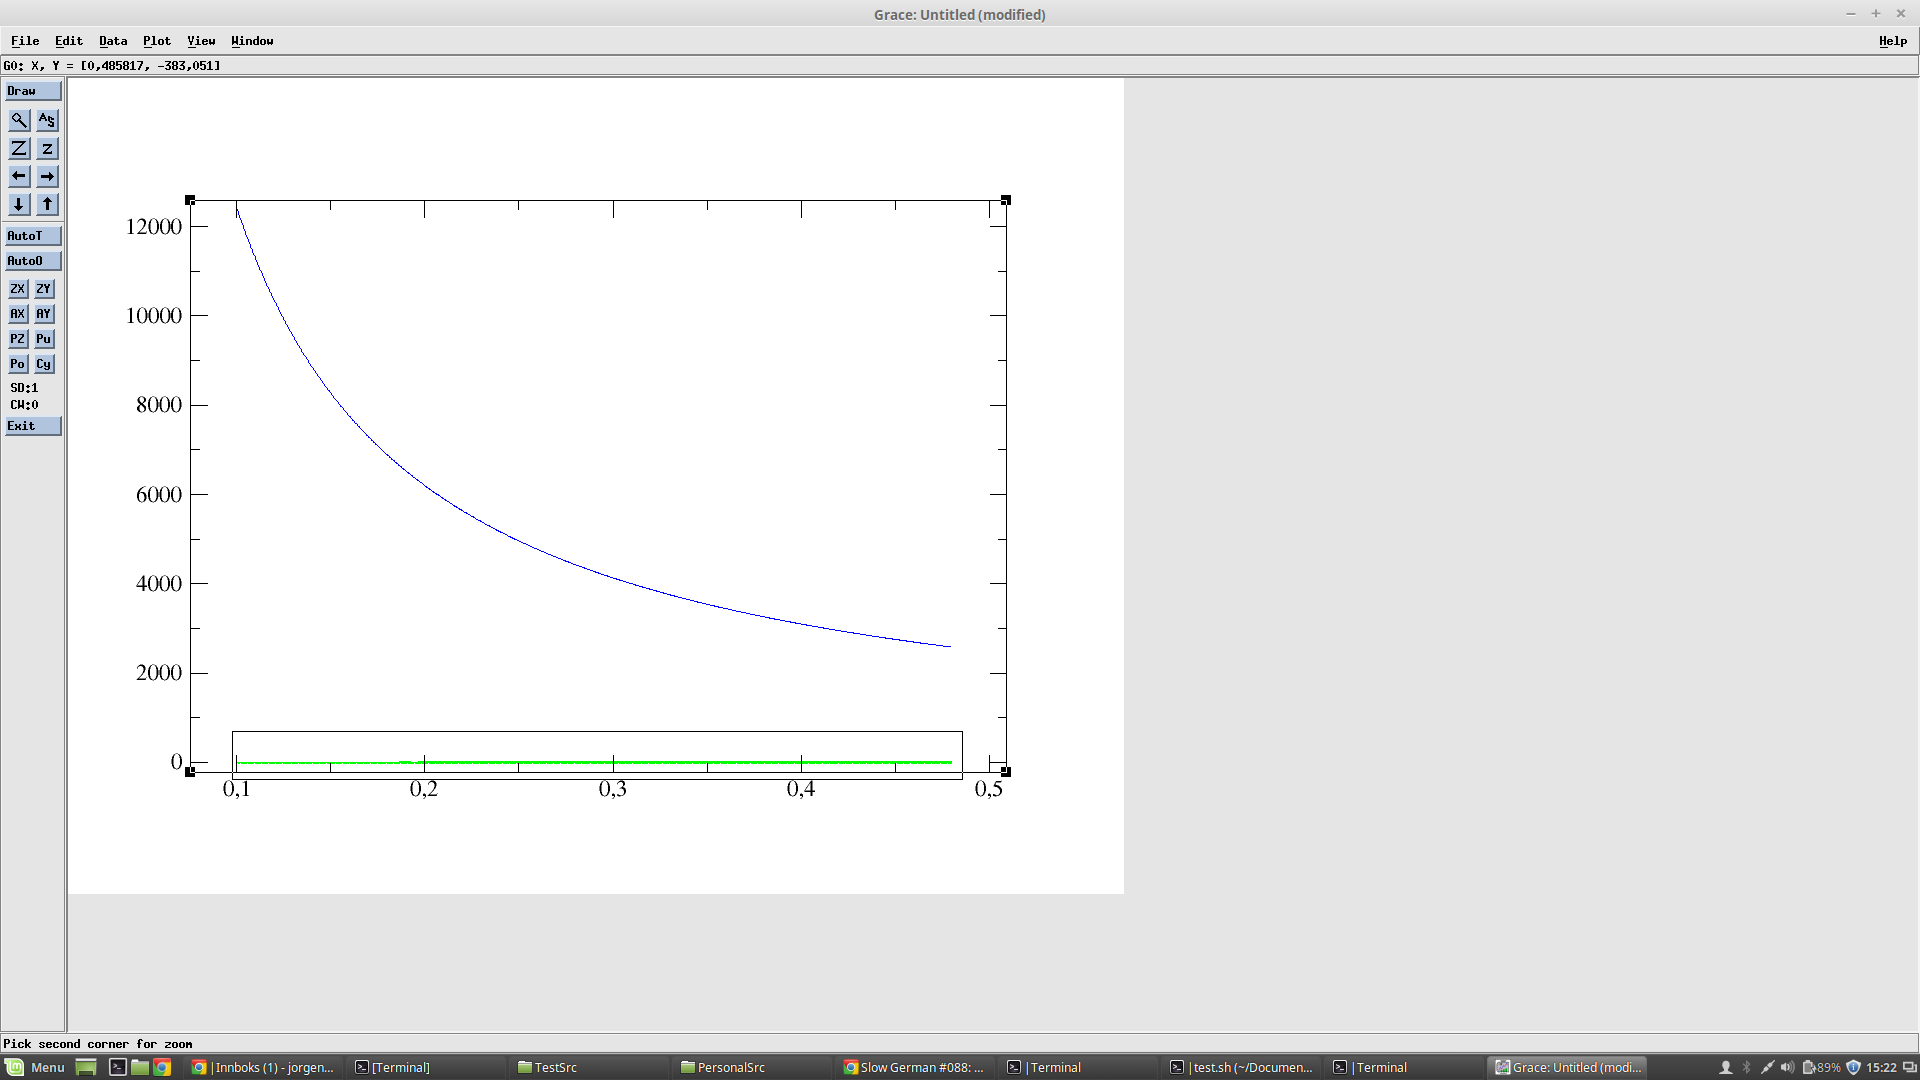
\includegraphics[width=1.0\textwidth]{Figures/result1a.png} 
      \caption{}
      \label{fig1}
      \end{figure}
      %
      \begin{figure}[h!] 
      \centering 
      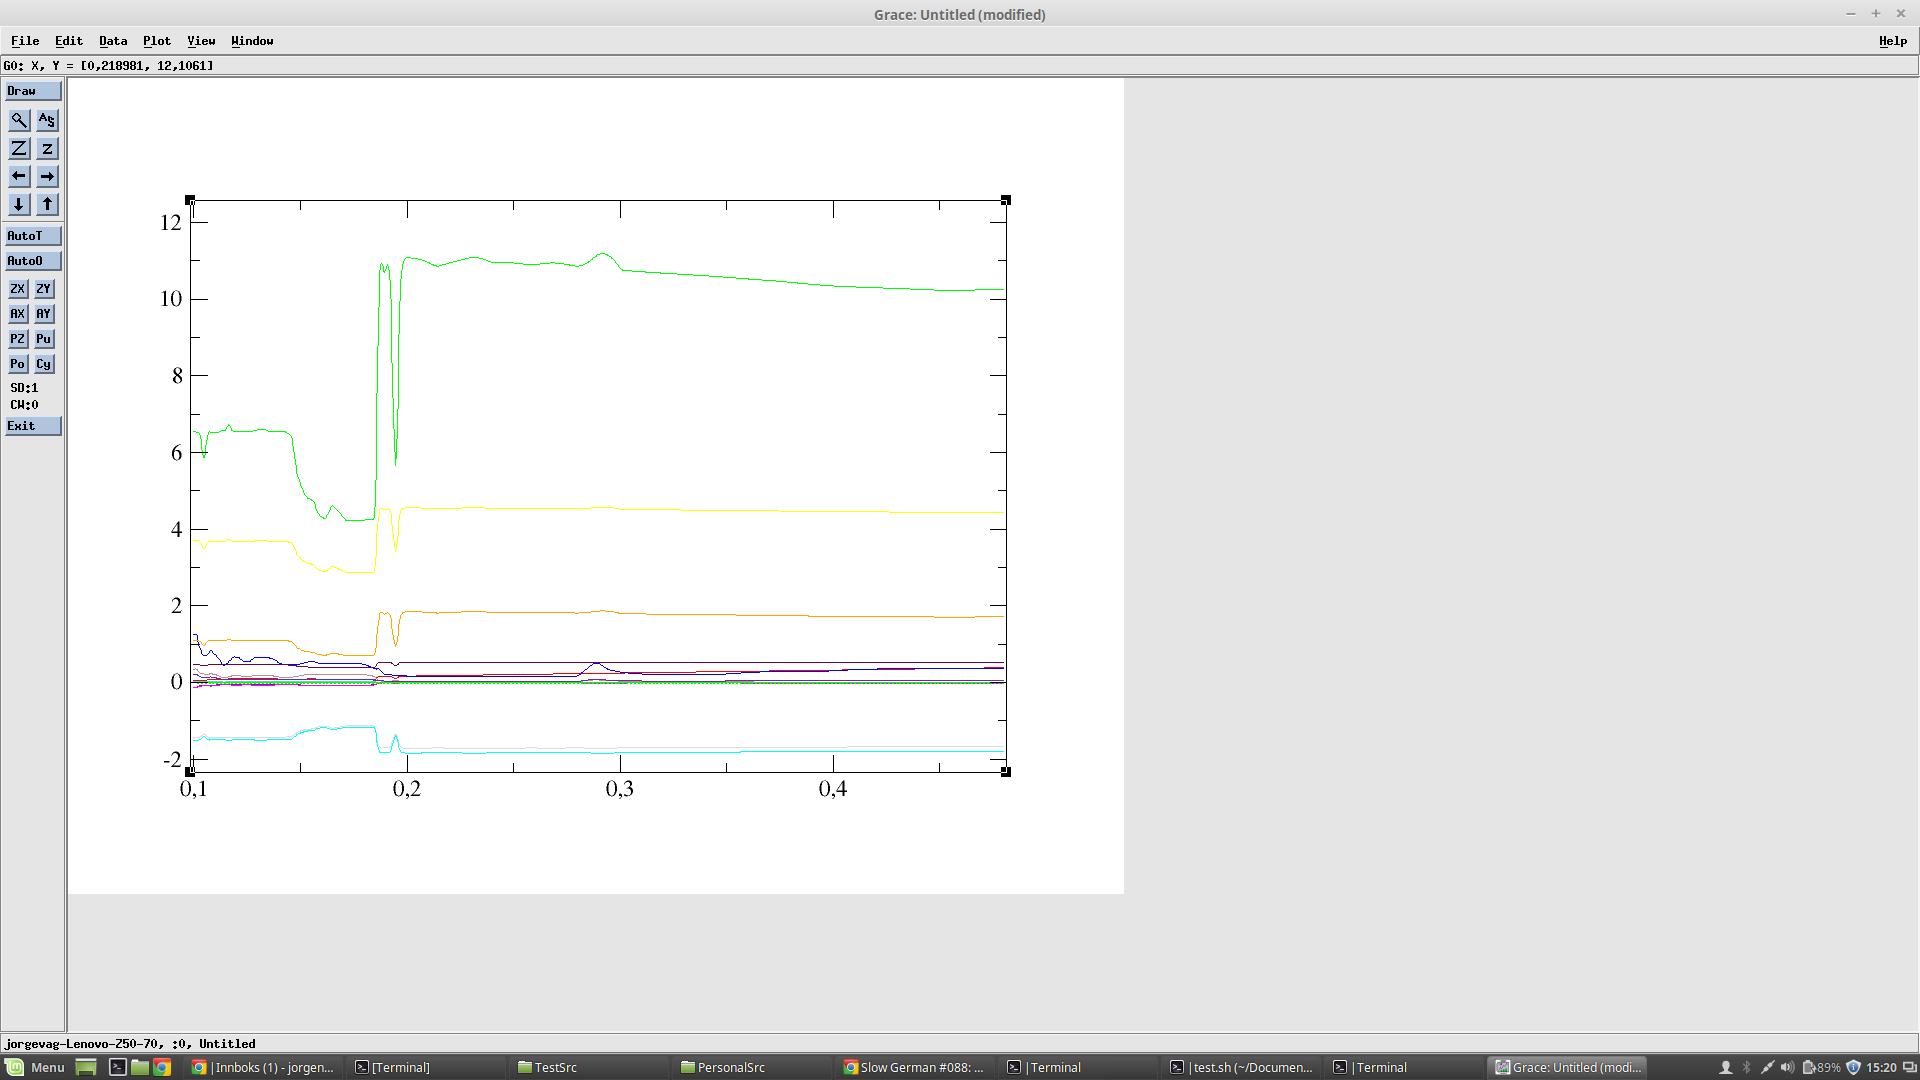
\includegraphics[width=1.0\textwidth]{Figures/result1b.png} 
      \caption{}
      \label{fig2}
      \end{figure}
      %
      \begin{figure}[h!] 
      \centering 
      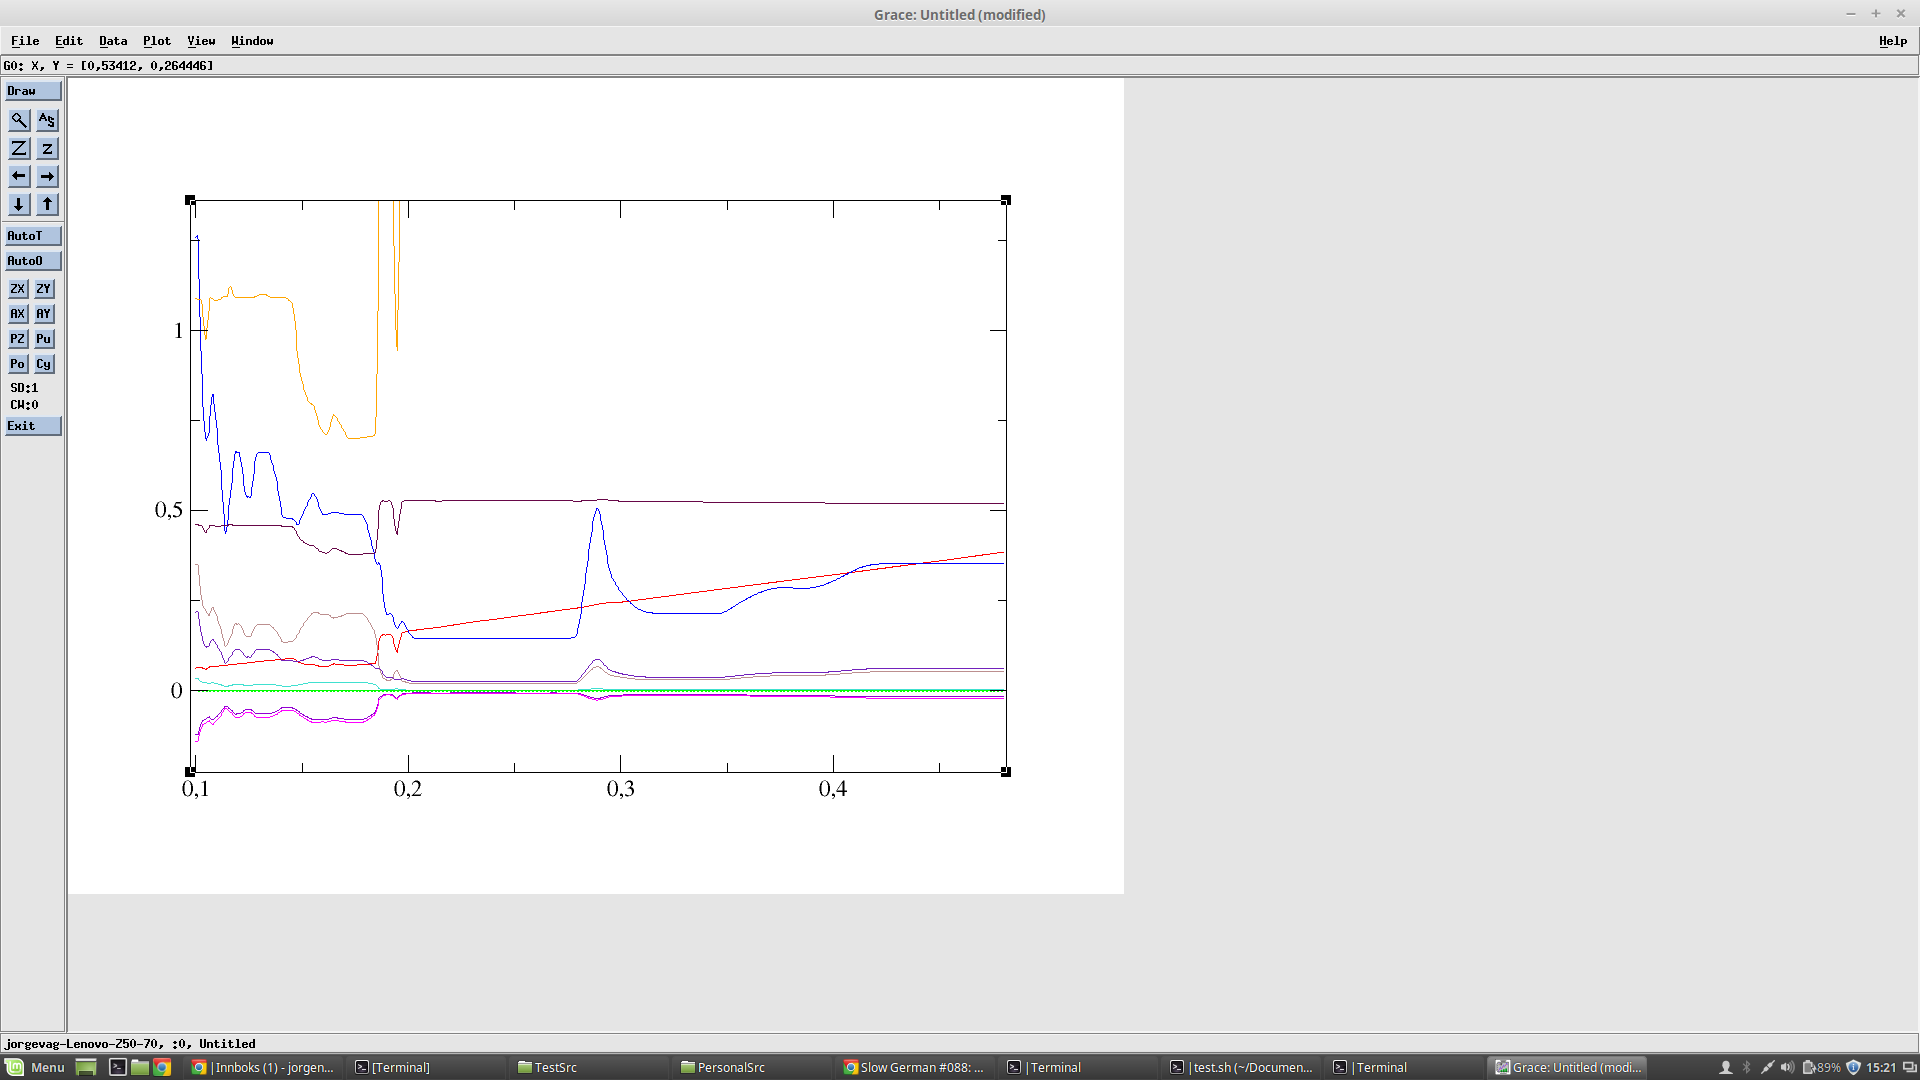
\includegraphics[width=1.0\textwidth]{Figures/result1c.png} 
      \caption{}
      \label{fig3}
      \end{figure}


\end{enumerate}
